\chapter{Mérések} \label{chapter5}

A webes alkalmazások kitelepítése hagyományosan szerverek felállításával, bekonfigurálásával és kezelésével járt, viszont a felhőalapú technológiák rohamos fejlődése egy alternatív megközelítést vezetett be: a \textit{serverless} megközelítéseket. Ennek a fejezetnek az a célja, hogy összehasonlítsa a \textit{serverless} telepítések teljesítmény- és költségmetrikáit a hagyományos szerver telepítésekével. 

A vizsgálat megvalósítása érdekében a \textit{Project Raccoon}-nak két változatát hoztuk létre: az egyiket Docker segítségével telepítettük ki, ami a hagyományos szerveres megközelítést képviseli, a másikat pedig \textit{serverless} technológiák segítségével, konkrétan a Vercel használatával.

A teljesítménymutatók, például a válaszidők, az erőforrás-kihasználás, valamint a költségmutatók körbejárásával a fejezet célja, hogy rávilágítson ezeknek a telepítési stratégiáknak az előnyeire és korlátaira.

Olyan információkat szeretnénk mutatni, melyek informálhatják a döntéshozatali folyamatot a fejlesztők számára a kitelepítést illetően.

Az összés mérést Marosvásárhelyen készítettük, egy AMD Ryzen 5 5600H-es számítógépen, 16 GB memóriával és 1000 megabites hálózati sávszélességgel. A hagyományos szerver Németországban van kitelepítve a Hetzner szolgáltatónál: egy CPX11 szerverről van szó.

A Docker-es megvalósítás elérhető a következő linken, illetve letölthető a diplomadolgozat mellékleteiből is: \url{https://raccoon.tohka.us}

A Vercel-es (\textit{serverless}) megvalósítás elérhető a következő linken: \url{https://raccoon.sallai.me}

\pagebreak

\section{Késleltetési teszt: hidegindítás esetén}

\begin{figure}[!h]
	\centering
        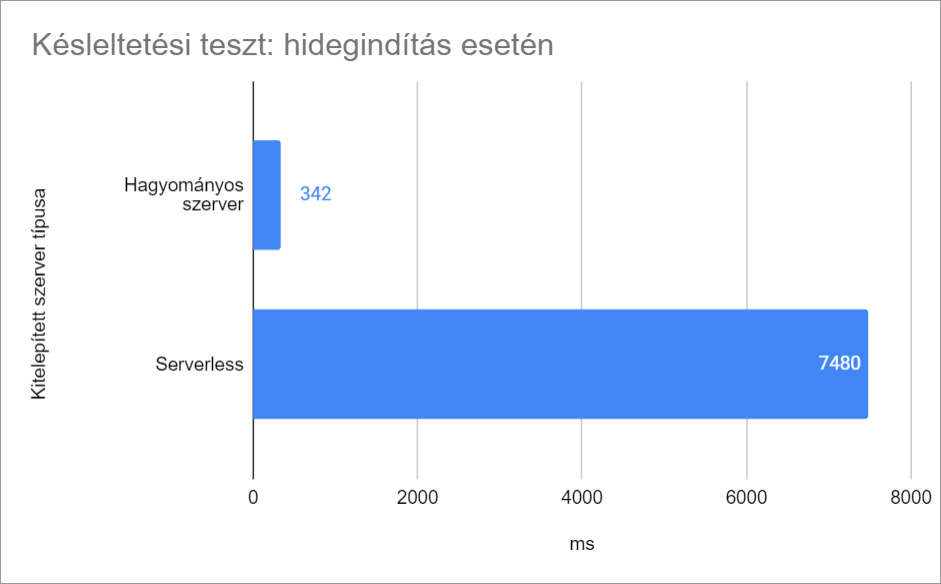
\includegraphics[scale=0.75]{images/measurement/diagram1.png}
	\caption{Késleltetési teszt: hidegindítás esetén}
        \label{measure:diagram1}
\end{figure}

A \ref{measure:diagram1}. ábrán látható a késleltetési teszt eredményei hidegindítás esetén. A tesztet 10-szer hajtottuk végre. A teszt során egy Python program segítségével lemértük, mennyi időbe kerül, hogy válaszoljon a weboldal. Az eredményeket átlagoltuk. A futtatások között vártunk 10 percet, annak érdekében, hogy a serverless környezetben futtatott alkalmazás kikerüljön a meleg futtatási környezetéből.

Látható, hogy a serverless weboldalnak jelentősen több időbe kerül válaszolnia a hidegindítás során a kérésekre. Ez azzal magyarázható, hogy a felhőben a szerver le kell töltse a futtatás előtt a futtatandó függvényeket. Ha fontos, hogy mindig egyből elérhető legyen az alkalmazásunk, válasszuk a hagyományos szervert.

\pagebreak

\section{Késleltetési teszt: melegindítás esetén}

\begin{figure}[!h]
	\centering
        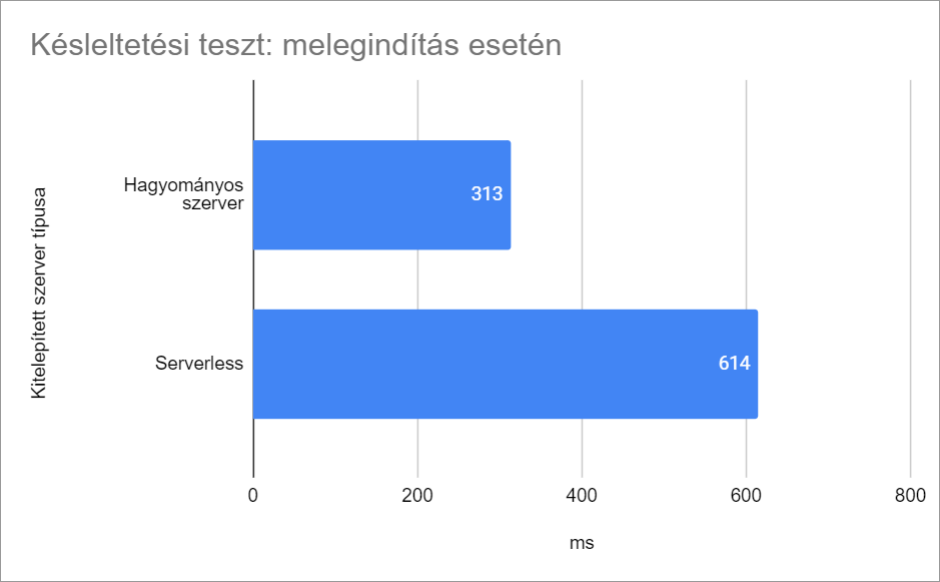
\includegraphics[scale=0.75]{images/measurement/diagram2.png}
	\caption{Késleltetési teszt: melegindítás esetén}
        \label{measure:diagram2}
\end{figure}

A \ref{measure:diagram2}. ábrán látható a késleltetési teszt eredményei melegindítás esetén. Hasonlóképpen az előző tesztet, egy Python program segítségével lemértük, hogy mennyi időbe kerül az alkalmazás válasza a kéréseinkre. A weboldal főlapját kértük el, hitelesítés nélkül. A tesztet 100-szor futtattuk le, egymás után, várakozás nélkül. Az első 5 eredményt elvetettük, a többit átlagoltuk.

Ha összehasonlítjuk az eredményeket a \ref{measure:diagram1}. 
ábrával, észrevehetjük, hogy nem létezik különösebb különbség a késleltetés szempontjából a meleg és hideg indítások során a hagyományos szervereknél.

A \ref{measure:diagram2} ábrát nézve megfigyelhetjük, hogy bár a hagyományos szerver Németországban van kitelepítve, a hagyományos szerver kevesebb késleltetésben szenved mint a serverless megoldás. 

\pagebreak

\section{Telepítési idő frissítéskor}

\begin{figure}[!h]
	\centering
        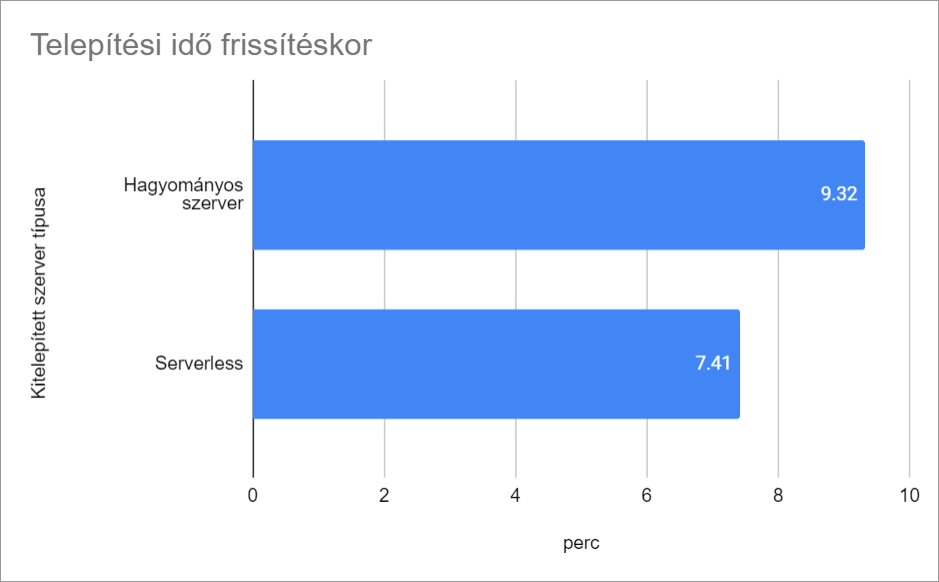
\includegraphics[scale=0.75]{images/measurement/diagram3.png}
	\caption{Telepítési idő frissítéskor}
        \label{measure:diagram3}
\end{figure}

A \ref{measure:diagram3}. ábrán látható a telepítési teszt eredményei frissítéskor. A Vercel platformról a legutolsó 5 telepítés idejét vettük a serverless adatoknak, míg a hagyományos szerverek esetében lefuttattuk ötször a Docker buildelési és telepítési folyamatát. A telepítési időket átlagoltuk.

A serverless platform majdnem két egész perccel gyorsabb a hagyományos szervernél. A hagyományos szerver telepítésének lassúsága magyarázható azzal, hogy a Hetzneres szerver, amelyre telepítettük a rendszert, csupán egy CPX11 instance: két CPU core-al rendelkezik, ami nem segíti elő egyáltalán a párhuzamos telepítési folyamatot.

Ha gyorsabb telepítést szeretnénk, akkor mindenképp válasszunk serverless megoldást.

\pagebreak

\section{Költségelemzés havonta: alacsony használati előrejelzés}

\begin{figure}[!h]
	\centering
        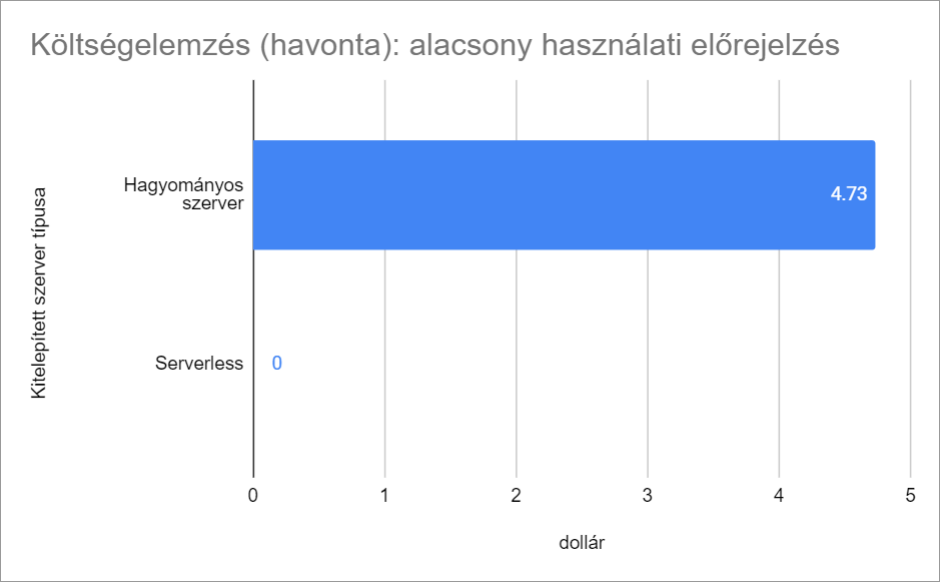
\includegraphics[scale=0.75]{images/measurement/diagram4.png}
	\caption{Költségelemzés havonta: alacsony használati előrejelzés}
        \label{measure:diagram4}
\end{figure}

A \ref{measure:diagram4}. ábrán látható a költségelemzés alacsony használati előrejelzésre. A költségelemzésünk egyszerű volt ebben az esetben: a hagyományos szervernek egy Hetzner CPX11 szervert választottunk, míg a serverless megoldásnak a Vercel ingyenes \textit{free tierjét} választottuk.

Mivel a Vercel teljesen ingyenesen használható 500,000 kérésig, ezért alacsony használat esetében teljesen ingyenes. A hagyományos szerver futtatása viszont pénzbe kerül: pontosan 4.73 dollárba. Ha nagyon kevés felhasználónk van, nincs értelme egy egész szervert kibérelni.

\pagebreak

\section{Költségelemzés havonta: magas használati előrejelzés}

\begin{figure}[!h]
	\centering
        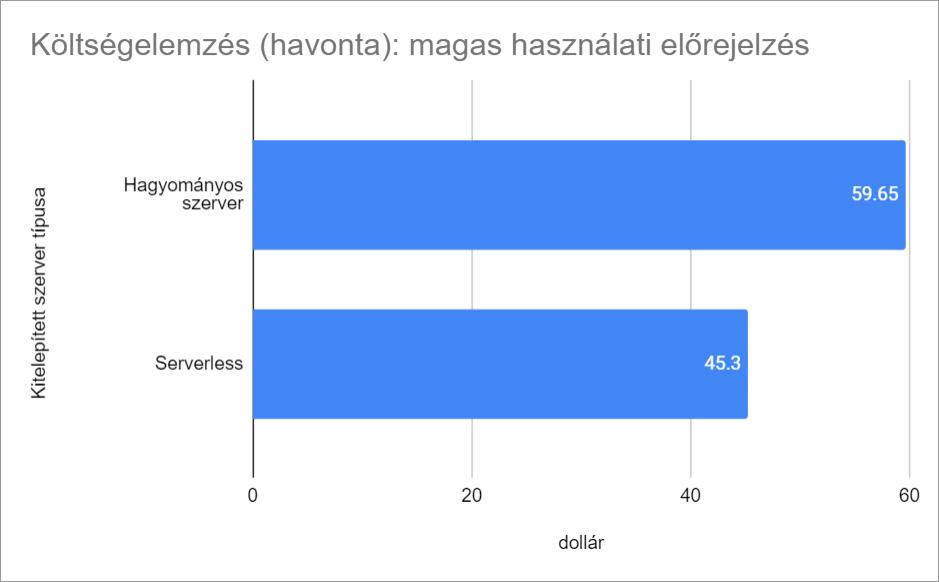
\includegraphics[scale=0.75]{images/measurement/diagram5.png}
	\caption{Költségelemzés havonta: magas használati előrejelzés}
        \label{measure:diagram5}
\end{figure}

A \ref{measure:diagram5}. ábrán látható a költségelemzés magas használati előrejelzésre.  A költségelemzésünk itt már komplikáltabb. Hagyományos szervernek a Hetzner CPX51 szerverét választottuk. Ennek költségét nagyon könnyű kiszámítani – egyetlen összetevőről van szó.

Serverless kontextusban sokkal bonyolultabbak a számítások. A serverless világban kell fizetni a programozók számáért is, a kérések számáért, illetve a sávszélességért is. 3 millió kérésben gondolkodtunk, 2 programozóban és 1 terabyte sávszélességben. Mivel egy felhasználó 20 dollárba kerül havonta, illetve 1 millió után minden millió kérés után 2.65 dollárt kér a Vercel, ezért a végeredmény 59.65 dollár.

Ha nem szeretnénk túlkomplikálni az életünket hasonló számítgatásokkal, jobban megéri a hagyományos szerver, amelynek futtatási költségei mindig konstansak maradnak.